% Stage 2: Ontology-Guided Extraction vs Baseline Comparison Figure
% This figure illustrates the difference between traditional extraction and ontology-guided extraction

\begin{figure*}[t]
\centering
\begin{tikzpicture}[
    node distance=0.8cm and 1.2cm,
    box/.style={rectangle, draw, rounded corners, minimum width=2.2cm, minimum height=0.7cm, align=center, font=\small},
    process/.style={box, fill=blue!15},
    data/.style={box, fill=green!15},
    output/.style={box, fill=orange!15},
    error/.style={box, fill=red!15, draw=red},
    success/.style={box, fill=green!20, draw=green!60!black},
    arrow/.style={->, >=stealth, thick},
    dashedarrow/.style={->, >=stealth, dashed, gray},
    label/.style={font=\footnotesize\itshape, text=gray},
]

% ===== BASELINE APPROACH (Left Side) =====
\node[font=\bfseries] at (-4.5, 4.5) {(a) Baseline Extraction};

% Input
\node[data] (pdf1) at (-4.5, 3.5) {PDF Document};

% Process
\node[process] (llm1) at (-4.5, 2.2) {LLM Extraction\\(Unstructured)};

% Outputs - showing fragmented results
\node[error] (out1a) at (-6.2, 0.8) {\footnotesize ``GHG emissions\\metric''};
\node[error] (out1b) at (-4.5, 0.8) {\footnotesize ``Energy use\\total''};
\node[error] (out1c) at (-2.8, 0.8) {\footnotesize ``Water\\consumed''};

% Problems
\node[error, minimum width=4.5cm] (prob1) at (-4.5, -0.7) {\footnotesize Inconsistent terminology};
\node[error, minimum width=4.5cm] (prob2) at (-4.5, -1.6) {\footnotesize No semantic relationships};
\node[error, minimum width=4.5cm] (prob3) at (-4.5, -2.5) {\footnotesize Missing calculation logic};

% Arrows
\draw[arrow] (pdf1) -- (llm1);
\draw[arrow] (llm1) -- (out1a);
\draw[arrow] (llm1) -- (out1b);
\draw[arrow] (llm1) -- (out1c);
\draw[dashedarrow] (out1a) -- (prob1);
\draw[dashedarrow] (out1b) -- (prob1);
\draw[dashedarrow] (out1c) -- (prob1);

% ===== ONTOLOGY-GUIDED APPROACH (Right Side) =====
\node[font=\bfseries] at (4.5, 4.5) {(b) Ontology-Guided Extraction};

% Input
\node[data] (pdf2) at (4.5, 3.5) {PDF Document};

% Ontology constraint
\node[process, fill=purple!20] (onto) at (7.2, 2.2) {ESG Ontology\\Schema};

% Process with ontology guidance
\node[process] (llm2) at (4.5, 2.2) {LLM Extraction\\+ Ontology Constraints};

% Structured outputs
\node[success] (cat) at (2.5, 0.6) {\footnotesize \textbf{Category}\\GHG Emissions};
\node[success] (met) at (4.5, 0.6) {\footnotesize \textbf{Metric}\\Scope1Emissions};
\node[success] (mod) at (6.5, 0.6) {\footnotesize \textbf{Model}\\GHGIntensity};

% Semantic relationships
\node[success, minimum width=5cm] (rel1) at (4.5, -0.7) {\footnotesize Category $\xrightarrow{consistsOf}$ Metric};
\node[success, minimum width=5cm] (rel2) at (4.5, -1.6) {\footnotesize Metric $\xrightarrow{isCalculatedBy}$ Model};
\node[success, minimum width=5cm] (rel3) at (4.5, -2.5) {\footnotesize Model $\xrightarrow{requiresInputFrom}$ DataPoint};

% Arrows
\draw[arrow] (pdf2) -- (llm2);
\draw[arrow, purple] (onto) -- (llm2);
\draw[arrow] (llm2) -- (cat);
\draw[arrow] (llm2) -- (met);
\draw[arrow] (llm2) -- (mod);
\draw[arrow, green!60!black] (cat) -- (rel1);
\draw[arrow, green!60!black] (met) -- (rel1);
\draw[arrow, green!60!black] (met) -- (rel2);
\draw[arrow, green!60!black] (mod) -- (rel2);

% Dividing line
\draw[thick, dashed, gray] (0, 4.8) -- (0, -3.2);

% Legend at bottom
\node[label] at (-4.5, -3.5) {Fragmented, unstructured output};
\node[label] at (4.5, -3.5) {Semantically structured knowledge graph};

\end{tikzpicture}

\caption{Comparison of extraction approaches in Stage 2. (a) Baseline extraction produces fragmented entities with inconsistent terminology and no semantic relationships. (b) Ontology-guided extraction uses the ESG ontology schema to constrain LLM outputs, producing structured entities with explicit semantic relationships (e.g., \texttt{consistsOf}, \texttt{isCalculatedBy}, \texttt{requiresInputFrom}) that enable downstream reasoning and calculation.}
\label{fig:stage2_comparison}
\end{figure*}
